\chapter{Materials and Methods}

\section{Dataset}
\label{sec:dataset}
We collected a set of $1\,592\,385$ anatomopathological exam results
from Tuscany region \ac{rtt} in the period 2004-2013. About $6\%$
of these records refer to a positive tumor
diagnosis and have topological and morphological ICD-O3 labels,
determined by tumor registry experts. Other reports are associated
with non-cancerous tissues and with unlabeled records. When multiple
pathological records for the
same patient existed for the same tumor, experts selected the most
informative report in order to assign the ICD-O3 code to that tumor
case, leaving a set of $94\,524$ labeled tumor cases.

The histological exam records consist of three free-text fields (not all
of them always filled-in) reporting tissue macroscopy, diagnosis,
and, in some cases, the patient's anamnesis. We found that field
semantics was not always used consistently and that the amount of
provided details varied significantly from extremely synthetic to very
detailed assessments of the morphology and the diagnosis. Field length
ranged from $0$ to $1\,368$ words, with first quartile, median and
third quartile respectively 34, 62, 134. For these reasons, we merged
the three text fields
into a single text document. We did not apply any conflation (except for
case normalization) kept punctuation.


We also collected the remaining unlabeled part of the dataset to train
unsupervised methods.

\subsection{Preparation}
The data used in this work comes from the \ac{rtt}. Originally, it
comes in two tables. The first one is composed of
a list of
neoplasm records, for each one are specified: a series of
administrative variables, e.g.\ the date of incidence, the hospital;
\ac{icdo} codes, both first and third editions, for topography and
morphology; other clinical variables, e.g.\ \emph{Gleason},
\emph{Clark}, \emph{Dukes} scores.
\ac{icdo} codes inside neoplasm records are assigned by
\ac{rtt} personnel, thus they can be considered reliable and used as
ground truth for the learning models.

Furthermore, there is a histology table containing records resulting
from microscopy exams. Each record contains three free-text
fields: one for the macroscopy, one for the diagnosis, and one for
other information.
% Besides, the histology table contains \ac{icdo} and
% \ac{icdo3} codes resulting from the application of the preexisting
% rule-based classifier. We employ these codes in order to assess the
% existing
% system, and use it as a baseline.

The neoplasm and histology tables can be joined using a
neoplasm identifier. Thus connecting the text
fields with the true \ac{icdo} codes.

%The data set is composed of $309\,852$ neoplasm and $1\,592\,385$
%histology records. When joined, the resulting records are $94\,524$.

There are neoplasm cases
without a related histology exam because \ac{rtt} uses also other
sources to collect tumor cases, e.g.\ \acp{hdr} and death
certificates. There are also histology exams without a related
neoplasm 
case because not always a histology results in a tumor case.

To train the unsupervised methods, we kept all the records from the
histology table that cannot be joined with 
the neoplasm table.

\section{Models}\label{sec:models}
In total, we created thirteen models:
\begin{description}
\item[\svm] uses \ac{svm} trained on \ac{tfidf} representations of text
  using unigrams;
\item[\svmb] uses \ac{svm} trained on \ac{tfidf} representations
  using unigrams and bigrams;
\item[\lstmng] uses \ac{lstm} layers trained on \ac{tfidf} representations using
  bigrams;
\item[\lstmc] uses mixed convolutional and \ac{lstm} layers trained on
  \ac{glove} representations;
\item[\lstmb] uses \ac{lstm} trained on \ac{glove} representations;
\item[\gru] uses \ac{gru} layers trained on \ac{glove} representations;
\item[\maxp] uses \ac{gru} layers with max pooling trained on \ac{glove}
  representations;
\item[\softmax] uses \ac{gru} layers with attention trained on \ac{glove}
  representations;
\item[\maxi] uses \ac{gru} layers with max pooling, in an interpretable setting, trained on \ac{glove}
  representations;
\item[\softmaxi] uses \ac{gru} layers with attention, in an interpretable setting, trained on \ac{glove}
  representations;
\item[\maxh] uses hierarchical \ac{gru} layers with max pooling trained on \ac{glove}
  representations;
\item[\softmaxh] uses hierarchical \ac{gru} layers with attention trained on \ac{glove}
  representations;
\item[\bert] is the model in \cite{devlin2018bert} pretrained
  on our unlabeled data and fine tuned with our labeled data.
\end{description}

In models \svm{} and \svmb{}, we used a \ac{tfidf}
representation ignoring terms present in less
than 3 documents or in
more than 30\% of the documents. 

We trained all the models except \ac{svm} minimizing
the \emph{categorical crossentropy}.

In \lstmng{} we used a word embedding of $30$. The
embedding layer corresponds to a one-hot representation of the input
followed by a dense layer of $30$ neurons.

\begin{figure}
  \centering
  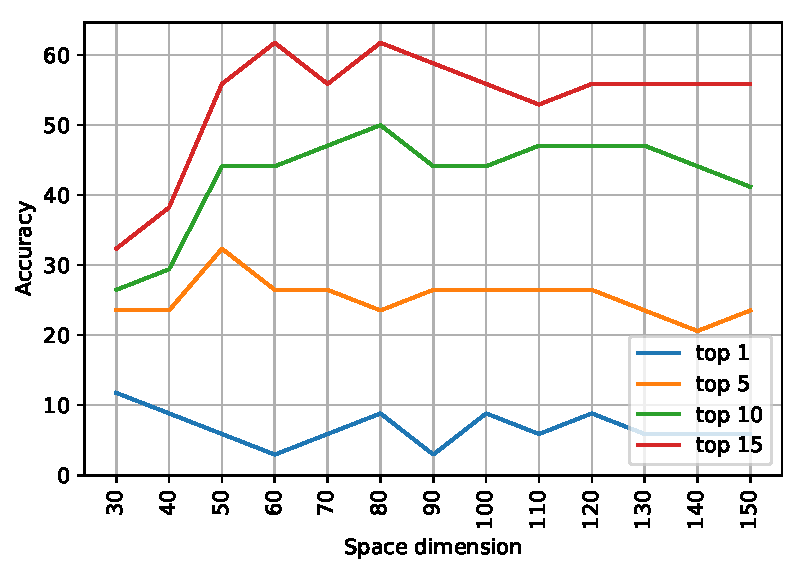
\includegraphics[width=0.45\textwidth]{img/gloveParameter.pdf}
  \caption{Accuracy top 1,5,10 and 15 for an intrinsic test with
    varying word vector dimension.}
  \label{fig:gloveParameter}
\end{figure}
In \lstmb{} and \lstmc{} we used the word vector representation
explained in \cref{sec:word-vectors}. We trained \ac{glove} with a window dimension of $15$,
in $50$ iterations to produce representations in dimension $60$. To
decide these parameters, we developed intrinsic tests collecting
quadruples like:
$$
(melanoma,\ cute,\ duttale,\ mammella)
$$
translated:
$$
(melanoma,\ skin,\ ductal,\ breast)
$$
in order to verify if $\vect{x}_{breast}$ is near
$\vect{x}_{skin}-\vect{x}_{melanoma}+\vect{x}_{ductal}$. Then we
proceeded to confront the different parameters as in
\cref{fig:gloveParameter}.

In order to accelerate the computation for the models \lstmng{}, \lstmb{}
and \lstmc{}, we cut the length of text to 200. The
$87\%$ of records have less than 200 words.

\lstmng{} is the \ac{ann} in \cref{fig:schemeLstmng}. It is
composed of two layers of $150$ bidirectional \ac{lstm} cells,
followed by an average pooling of the sequences, followed by a
dense \ac{relu} layer, followed by a dense \emph{softmax} layer.
The number of \acp{an} of the last two layers is
equal to the number of classes for each task.
\begin{figure}
  \centering
  \begin{tikzpicture}[node distance = 0.1cm, auto]
    \begin{scope}[start chain, every node/.style={on chain}, node distance = \schemeNodeDistance]
      \nodeInput();
      \nodeEmbedding();
      \node[support] (emb) {};
      \nodeLstm();
      \node[support] (lstmA) {};
      \nodeLstm();
      \node[support] (lstmB) {};
      \nodeAvg();
      \node[support] (avg) {};
      \nodeRelu();
      \node[support] (relu) {};
      \nodeSoftmax();
      \node[dataLabel, joined] {$outDim$};
    \end{scope}
    \node[dataLabel, above=of emb] {$200\times 30$};
    \node[dataLabel, above=of lstmA] {$200\times 300$};
    \node[dataLabel, above=of lstmB] {$200\times 300$};
    \node[dataLabel, above=of avg] {$300$};
    \node[dataLabel, above=of relu] {$outDim$};
  \end{tikzpicture}
  \caption{Scheme for \lstmng{} model.}
  \label{fig:schemeLstmng}
\end{figure}

\lstmc{}, in \cref{fig:schemeLstmc}, is composed of a convolutional
filter of size two, followed by a bidirectional \ac{lstm} layer of
$150$ cells, followed by an average pooling of the sequences,
followed by a dense \ac{relu}, followed by a dense \emph{softmax}
layer.
\begin{figure}
  \centering
  \begin{tikzpicture}[node distance = 0.1cm, auto]
    \begin{scope}[start chain, every node/.style={on chain}, node distance = \schemeNodeDistance]
      \nodeInput();
      \nodeGlove();
      \node[support] (glove) {};
      \nodeConv();
      \node[support] (conv) {};
      \nodeLstm();
      \node[support] (lstm) {};
      \nodeAvg();
      \node[support] (avg) {};
      \nodeRelu();
      \node[support] (relu) {};
      \nodeSoftmax();
      \node[dataLabel, joined] {$outDim$};
    \end{scope}
    \node[dataLabel, above=of glove] {$200\times 60$};
    \node[dataLabel, above=of conv] {$199\times 100$};
    \node[dataLabel, above=of lstm] {$199\times 300$};
    \node[dataLabel, above=of avg] {$300$};
    \node[dataLabel, above=of relu] {$outDim$};
  \end{tikzpicture}
  \caption{Scheme for \lstmc{} model.}
  \label{fig:schemeLstmc}
\end{figure}

\lstmb{}, in \cref{fig:schemeLstmb}, is composed of two bidirectional
\ac{lstm} layer of 
$150$ cells, followed by an average pooling of the sequences,
followed by a dense \ac{relu}, followed by a dense \emph{softmax}
layer. 
\begin{figure}
  \centering
  \begin{tikzpicture}[node distance = 0.1cm, auto]
    \begin{scope}[start chain, every node/.style={on chain}, node distance = \schemeNodeDistance]
      \nodeInput();
      \nodeGlove();
      \node[support] (glove) {};
      \nodeLstm();
      \node[support] (lstmA) {};
      \nodeLstm();
      \node[support] (lstmB) {};
      \nodeAvg();
      \node[support] (avg) {};
      \nodeRelu();
      \node[support] (relu) {};
      \nodeSoftmax();
      \node[dataLabel, joined] {$outDim$};
    \end{scope}
    \node[dataLabel, above=of glove] {$200\times 60$};
    \node[dataLabel, above=of lstmA] {$200\times 300$};
    \node[dataLabel, above=of lstmB] {$200\times 300$};
    \node[dataLabel, above=of avg] {$300$};
    \node[dataLabel, above=of relu] {$outDim$};
  \end{tikzpicture}
  \caption{Scheme for \lstmb{} model.}
  \label{fig:schemeLstmb}
\end{figure}

\gru{} is a stacked bidirectional \ac{gru} model.

The other models where trained on different hyperparameters
configurations whose range is explained in
\cref{sec:hyperparameters}. We proceed to explain in detail their
structure.
\subsection{\maxp, \softmax, \maxi, \softmaxi}
\label{sec:model}
In our setting, a dataset $\mathcal{D}=\{(\vect{x}^{(i)},y^{(i)})\}$
consists of variable length sequence vectors $\vect{x}^{(i)}$. For
$t=1,\dots,T^{(i)}$, $x^{(i)}_t$ is the $t$-th word in the $i$-th
document and $y^{(i)}\in\{1,\dots,K\}$ is the associated target
class. To simplify the notation in the subsequent text, the
superscripts are not used unless necessary. Sequences are
denoted in boldface. The RNN-based sequence classifiers used in
this work compute their predictions $f(\vect{x})$ as follows:
\begin{align}
  e_t &= E(x_t;\theta^e),\label{eq:embed}\\
  h^f_t &= F(e_t,h^f_{t-1};\theta^f),\label{eq:maxModelRL}\\  
  h^r_t &= R(e_t,h^r_{t+1};\theta^r),\label{eq:maxModelRR}\\
  u_t &= G(h_t;\theta^h),\label{eq:maxModelF}\\
  \phi &= A(\vect{h},\vect{u};\theta^a),\label{eq:aggregation}\\
  f(\vect{x}) &= g(\phi;\theta^c).\label{eq:maxModelC}
\end{align}
$E$ is an embedding function mapping words into $p$-dimensional real
vectors where embedding parameters $\theta_e$ can be either
pretrained and adjustable or fixed, see Section~\ref{sec:word-vectors}
below.  Functions $F$ and $R$ correspond to (forward and reverse)
dynamics that can be described in terms of several (possibly layered)
recurrent cells. Each vector $h_t$,
the concatenation of $h^f_t$ and $h^r_t$, can be interpreted as latent
representations of the information contained at position $t$ in the
document. $G$ is an additional \ac{mlp} mapping each latent vector into a
vector $u_t$ that can be seen as contextualized representation of the
word at position $t$. $A$ is an aggregation function that creates a
single $d$-dimensional representation vector for the entire sequence
and $g$ is a softmax layer. Possible choices for the aggregator
function include:
\begin{itemize}
\item $\phi=(h^f_T,h^r_1)$, which
  extracts the extreme latent representations; in principle, these may
  be sufficient since they depend on the whole sequence due to 
  bidirectional dynamics. However, note that this approach may require
  long-term dependencies to be effectively learned;
\item
  % $\phi = \sum_t a_t(\vect{u};\theta^a) h_t$,
  $\phi = \sum_t a_t(\vect{u};\theta^a) u_t$,
  using an attention mechanism as in~\cite{yang_hierarchical_2016}. In
  this case, (scalar) attention weights are computed as
  \begin{align*}
    c_t&=C(\vect{u};\theta^a),\\
    a_t(\vect{u};\theta^a) &= \frac{e^{\langle c, c_t\rangle}}
    {\sum_i{e^{\langle c, c_i\rangle}}},\\
  \end{align*}
  %$$
  %a_t(\vect{u};\theta^a) = \frac{e^{\langle \theta^a, u_t\rangle}}
  %{\sum_s{e^{\langle \theta^a, u_s\rangle}}}
  %$$
  where $C$ is a single layer that maps the representation $u_t$ of the
  word to a hidden representation $c_t$. Then, the importance of the word is
  measured as a similarity with a context vector $c$ that is learned
  with the model and can be seen as an embedded representation of an
  high level query as in memory networks \cite{sukhbaatar2015end};
\item $\phi = \max_t u_t$ where the maximum is taken element-wise
  along the sequence. This approach can be interpreted either as a
  simplified (parameter-less) attention mechanism, or a bag-layer as
  proposed in the context of multi-instance
  learning~\cite{tibo2017network}. In this case, each ``feature''
  $\phi_j$ will be positive if at least one of $u_{j,1},\dots,u_{j,T}$
  is positive. The resulting classifier will find it easy to create
  decision rules predicting a document as belonging to a certain class
  if a given set of contextualized word representations are present
  and another given set of contextualized word representations are
  absent in the sequence.
\end{itemize}

The parameters $\theta^f,\theta^r,\theta^h$, and $\theta^a$ (if
present) are determined by minimizing a loss function $\loss$
(categorical cross-entropy in our case) on training data:
\begin{equation}
  \hat \theta = \mathrm{arg}\min_\theta\sum_{(\vect{x},y)\in\mathcal{D}}\loss\left(y,f(\vect{x})\right),
\end{equation}
where $\theta=\theta^f\cup\theta^r\cup\theta^h\cup\theta^a$.

We call \maxp{} the model $f(\vect{x})$ when setting the aggregator
function $A$ equal to the max pooling $\max_t u_t$. When we use
the attention $\sum_t a_t(\vect{u};\theta^a) u_t$ instead, we call the
model \softmax{}.

The model is flexible enough to gain interpretability under certain
assumptions. If we remove the last layer in \eqref{eq:maxModelC},
the dimension of last layer in \eqref{eq:maxModelF}
needs to be equal to the
output dimension (in the experiments: $1$ for the artificial dataset,
$68$ for the site task, and $203$ for the 
morphology).
We hypothesized that, in this case, the values of
$u_t$ (or the weighted values $a_t(\vect{u};\sigma^a)u_t$, if we use the
attention as aggregator) collect information on the importance of the
area 
around $x_t$ for the purpose of classification task. This
information can be
used to interpret the model decision. We call \maxi{} this
interpretable setting when using the max aggregator, and \softmaxi{}
when using the attention.
% $e:\XSet\rightarrow\RSet^k$ is an embedding function that transforms
% sequence elements in tensors $\vect{x}_{i,j}=e(x_{i,j})$ of
% dimension $k$ that can be parsed by the
% model. $g:\YSet\rightarrow[0,1]^q$ is an embedding function that
% transforms sequences labels in one-hot encodings of a coherent
% dimension $q$.
\subsection{\maxh, \softmaxh}
\label{sec:modelh}
We extend the plain model of the previous section with a hierarchical setting,
similarly to other works \cite{yang_hierarchical_2016}. In this
setting our dataset $\mathcal{D}=\{\vect{x}^{(i)},y^{(i)}\}$
consists of variable length sequence of sequence vectors
$\vect{x}^{(i)}$, where, for $s=1,\dots,S^{(i)}$ and
$t=1,\dots,T^{(i,s)}$, $x_{s,t}^{(i)}$ is the $t$-th word of the $s$-th sentence in the
$i$-th document, and $y^{(i)}\in\{1,\dots,K\}$ is the associated
target class. The prediction $f(\vect{x})$ is calculated: 
\begin{align}
  e_{s,t} &= E(x_{s,t};\theta^e),\label{eq:embedH}\\
  h^f_{s,t} &= F(e_{s,t},h^f_{s,t-1};\theta^{f}),\label{eq:maxModelRLH}\\  
  h^r_{s,t} &= R(e_{s,t},h^r_{s,t+1};\theta^{r}),\label{eq:maxModelRRH}\\
  u_{s,t} &= G(h_{s,t};\theta^{h}),\label{eq:maxModelFH}\\
  \phi_s &= A(\vect{h}_s,\vect{u}_s;\theta^{a}),\label{eq:aggregationH}\\
  h'^{f}_{s} &= F'(\phi_{s},h'^{f}_{s-1};\theta'^{f}),\label{eq:maxModelRLHS}\\  
  h'^{r}_{s} &= R'(\phi_{s},h'^{r}_{s+1};\theta'^{r}),\label{eq:maxModelRRHS}\\
  \phi' &= A'(\vect{s},\vect{h}';\theta'^{a}),\label{eq:aggregationHS}\\
  f(\vect{x}) &= g(\phi';\theta^c).\label{eq:maxModelCH}
\end{align}
As in the plain model, $E$ is an embedding function, $F$ and $R$
correspond to forward and reverse dynamics that process word
representations,
$h_{s,t}=h_{s,t}^f\oplus h_{s,t}^r$ is the latent representation of
the information contained at position $t$ of the $s$-th sentence,
$u_{s,t}$ is the contextualized representation of the word at position
$t$ of the $s$-th sentence, and $A$ is an aggregation function that
creates a single representation for the sentence. Furthermore, $F'$ and
$R'$ correspond to 
forward and reverse dynamics that process sentence representations,
and $A'$ is the aggregation function that creates a single
representation for the entire document. $h'_s=h'^f_s\oplus h'^r_s$
can be interpreted as the
latent representation of the information contained in the sentence $s$
for the document.

We call \maxh{} and \softmaxh{} the hierarchical model when we use
respectively the max pooling and the attention.


%%% Local Variables:
%%% mode: latex
%%% TeX-master: "thesis"
%%% End:
